%%%%%%%%%%%%%%%%%%%%%%%%%%%%%%%%%%%%%%%%%%%%%%%%%%%%%
%                                                   %
%     Penn State Colloquium Poster Template         %
%                                                   %
% Uses Penn State Colloquium class, with options:   %
%                                                   %
% Orientation:                                      %
%     portrait (default), landscape                 %
%                                                   %
% Paper size:                                       %
%     a4paper (default), a0paper, a1paper, a2paper, %
%     a3paper, a5paper, a6paper                     %
%%%%%%%%%%%%%%%%%%%%%%%%%%%%%%%%%%%%%%%%%%%%%%%%%%%%%
\documentclass{../psuposter}
\renewcommand{\templateimagepath}{../} 


%%%%%%%%%%%%%%%%%%%%%%%%%%%%%%%%%%%%%%%%%%%%%%%%%%%%%
%               Package Dependencies                %
%%%%%%%%%%%%%%%%%%%%%%%%%%%%%%%%%%%%%%%%%%%%%%%%%%%%%
\usepackage{natbib}
\usepackage{lipsum}                                % Dummy text
\usepackage[figwidth = 0.98\linewidth]{todonotes}  % Dummy image (and more!)
\usepackage[absolute, overlay]{textpos}            % Figure placement
\usepackage{braket}
\setlength{\TPHorizModule}{\paperwidth}
\setlength{\TPVertModule}{\paperheight}
\setcitestyle{numbers,square}


%%%%%%%%%%%%%%%%%%%%%%%%%%%%%%%%%%%%%%%%%%%%%%%%%%%%%
%                 AUTHOR AND TITLE                  %
%%%%%%%%%%%%%%%%%%%%%%%%%%%%%%%%%%%%%%%%%%%%%%%%%%%%%
\title{Quantum Matter under the Microscope \newline
		\large{\textit{Engineering and Probing Quantum Matter using Quantum Simulations}}}
\author{Immanuel Bloch}
\institute{Ludwig Maximilians University}


%%%%%%%%%%%%%%%%%%%%%%%%%%%%%%%%%%%%%%%%%%%%%%%%%%%%%
%                  BEGIN DOCUMENT                   %
%%%%%%%%%%%%%%%%%%%%%%%%%%%%%%%%%%%%%%%%%%%%%%%%%%%%%
\begin{document}
\begin{frame}
\begin{columns}[t, totalwidth=\textwidth]
\begin{column}{0.45\textwidth - 1cm}


%%%%%%%%%%%%%%%%%%%%%%%%%%%%%%%%%%%%%%%%%%%%%%%%%%%%%
%                 BLOCK: BIOGRAPHY                  %
%%%%%%%%%%%%%%%%%%%%%%%%%%%%%%%%%%%%%%%%%%%%%%%%%%%%%
    \begin{block}{Speaker Biographic Summary}
    	\begin{center}
    		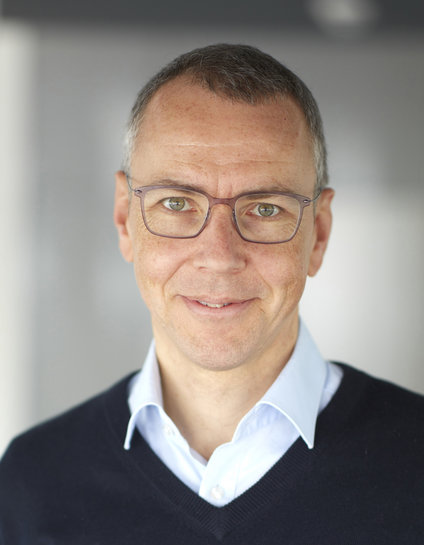
\includegraphics[width=0.58\textwidth]{images/bloch}
    	\end{center}
    	\href{https://www.quantum-munich.de/104554/bloch-immanuel-prof-dr}{Dr. Immanuel Bloch} is the scientific director at the Max-Planck-Institute of Quantum Optics and professor for experimental physics at the Ludwig-Maximilians University (LMU) in Munich, where he obtained his PhD in physics in 2000. Previously, he has held positions in the University of Mainz before returning to Munich. Immanuel Bloch received several prizes for his work, among them the Gottfried-Wilhelm-Leibniz prize of the German Science Foundation (DFG), the German National Merit Medal in 2005, the international commission of optics prize, the Senior Prize for Fundamental Aspects of Quantum Electronics and Optics of the European Physical Society, the Körber European Science Prize, the Senior BEC Award and the Harvey Prize of the Technion. 
    \end{block}


%%%%%%%%%%%%%%%%%%%%%%%%%%%%%%%%%%%%%%%%%%%%%%%%%%%%%
%            BLOCK: RESEARCH INTERESTS              %
%%%%%%%%%%%%%%%%%%%%%%%%%%%%%%%%%%%%%%%%%%%%%%%%%%%%%
    \begin{block}{Research Interests}
        Dr. Bloch's research interests focuses on quantum many-body systems, quantum simulations, quantum information processing and quantum optics. Bloch investigates properties of many-body systems using ultra cold atoms in optical lattices as simulations. He is known for the realization of a quantum phase transition from a superfluid to Mott insulator. \cite{weitenbergSinglespinAddressingAtomic2011} 
        More recently, his research team was able to realize single-atom resolved imaging and addressing of ultracold atoms held in an optical lattice. \cite{shersonSingleatomresolvedFluorescenceImaging2010}
        \begin{center}
	    	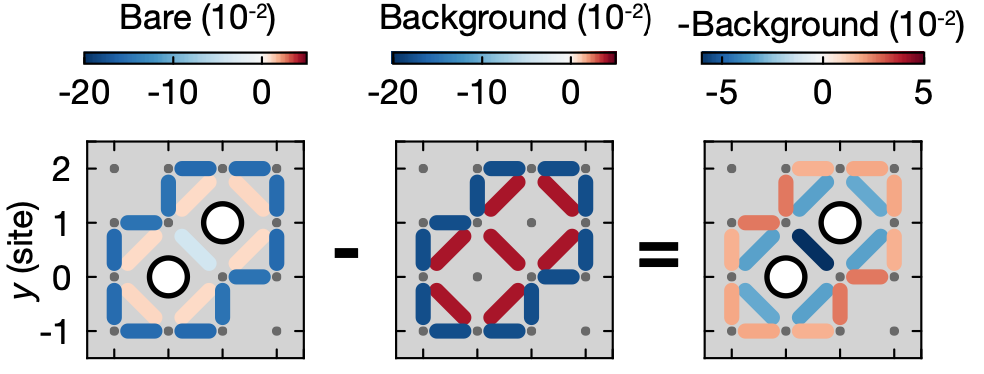
\includegraphics[width=0.75\textwidth]{images/diag-hole}    		
    	\end{center}
    	\textit{Decomposition of spin correlations, diagonal hole pair.} \cite{koepsellMicroscopicEvolutionDoped2020}
    \end{block}
\end{column}
\begin{column}{0.55\textwidth - 1cm}


%%%%%%%%%%%%%%%%%%%%%%%%%%%%%%%%%%%%%%%%%%%%%%%%%%%%%
%                 BLOCK: ABSTRACT                   %
%%%%%%%%%%%%%%%%%%%%%%%%%%%%%%%%%%%%%%%%%%%%%%%%%%%%%
    \begin{block}{Talk Abstract}
    	More than 30 years ago, Richard Feynman outlined his vision of a quantum simulator for carrying out complex calculations on physical problems. Today, his dream is a reality in laboratories around the world. This has become possible by using complex experimental setups of thousands of optical elements, which allow atoms to be cooled to Nanokelvin temperatures, where they almost come to rest. Recent experiments with quantum gas microscopes allow for an unprecedented view and control of artificial quantum matter in new parameter regimes and with new probes. In our atomic fermionic quantum gas microscope, we can detect both charge and spin degrees of freedom simultaneously, thereby gaining maximum information on the intricate interplay between the two in the Fermi Hubbard model. In my talk, I will show how we can reveal hidden magnetic order, directly image individual magnetic polarons, probe the fractionalisation of spin and charge in dynamical experiments and reveal the crossover from a polaronic metal to a Fermi liquid when continuously increasing the doping in the system. For the first time we thereby have access to directly probe non-local ‘hidden’ correlation properties of quantum matter and to explore its real space resolved dynamical features also far from equilibrium. Finally, I will discuss experiments on the first realization of the Haldane phase in Hubbard ladder systems. Both edge states and bulk string correlators enable us to reveal the special topological features of this paradigmatic phase of matter.
    \end{block}


%%%%%%%%%%%%%%%%%%%%%%%%%%%%%%%%%%%%%%%%%%%%%%%%%%%%%
%                BLOCK: BACKGROUND                  %
%%%%%%%%%%%%%%%%%%%%%%%%%%%%%%%%%%%%%%%%%%%%%%%%%%%%%
    \begin{block}{Brief Background}
    	Electrons interacting in conventional metals are described by Fermi-Liquid (FL) theory, which uses adiabaticity and the Pauli exclusion principle to relate the simple Fermi gas model to an interacting system. Violations of these concepts is a key feature of strongly-correlated quantum materials.
    	\cite{koepsellMicroscopicEvolutionDoped2020} 
        \begin{center}
		   	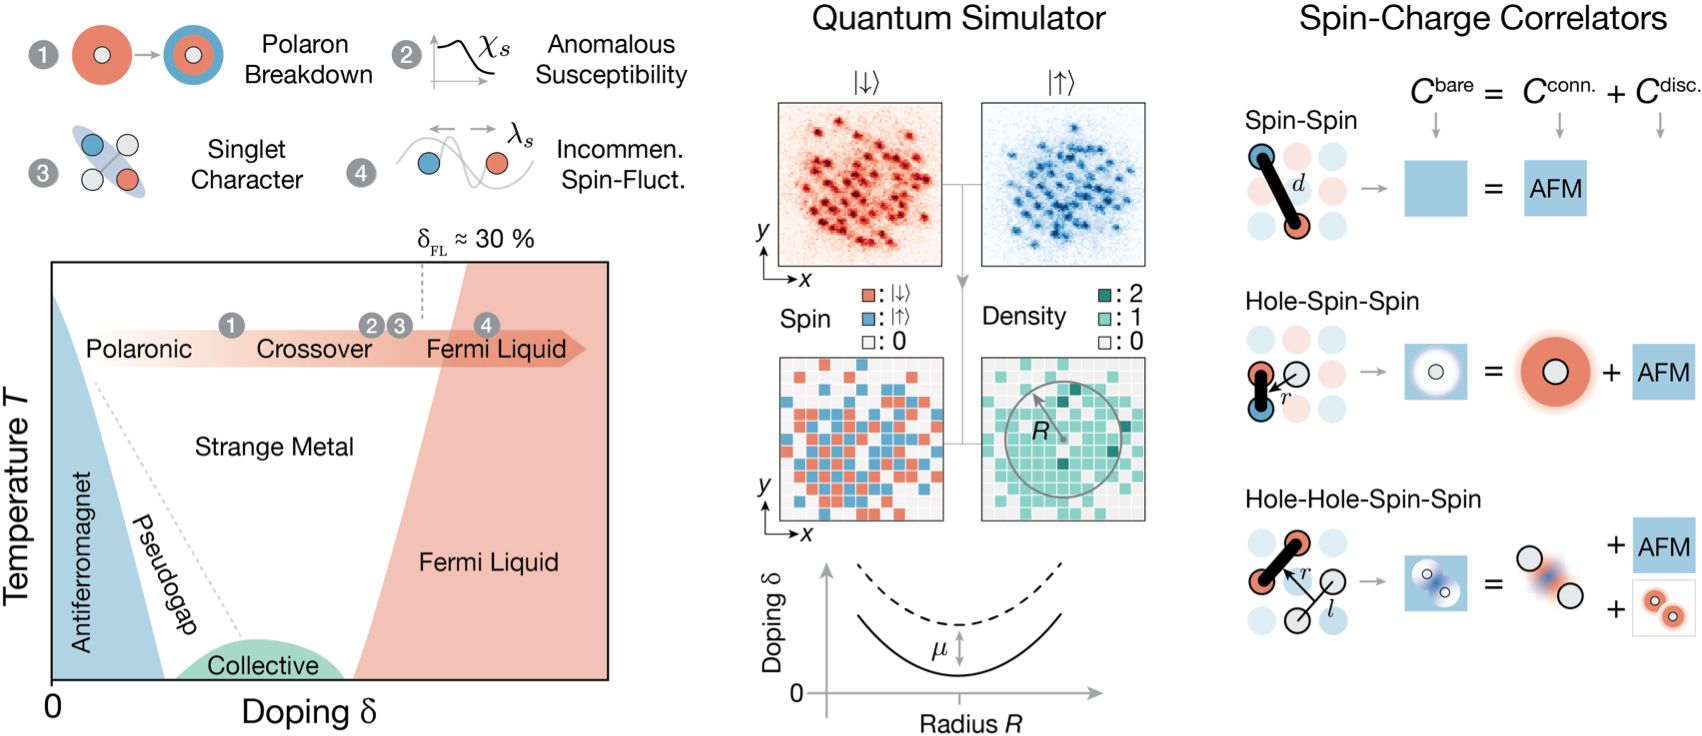
\includegraphics[width=0.8\textwidth]{images/mott-2}    		
    	\end{center}
		Doped antiferromagnetic Mott insulators are particularly interesting since they behave like non-FL materials for weak doping, but become normal FL materials for high doping. The combined effect of hole motion and antiferromagnetism produces magnetic polarons, or heavily dressed dopants.
		\cite{koepsellMicroscopicEvolutionDoped2020} 
    \end{block}


%%%%%%%%%%%%%%%%%%%%%%%%%%%%%%%%%%%%%%%%%%%%%%%%%%%%%
%                 BLOCK: REFERENCES                 %
%%%%%%%%%%%%%%%%%%%%%%%%%%%%%%%%%%%%%%%%%%%%%%%%%%%%%
    \begin{block}{References}
        \bibliographystyle{aipnum4-1}
%        \bibliographystyle{iopart-num}
		\bibliography{../references}
    \end{block}

\end{column}
\end{columns}


%%%%%%%%%%%%%%%%%%%%%%%%%%%%%%%%%%%%%%%%%%%%%%%%%%%%%
%                    FOOTER TEXT                    %
%%%%%%%%%%%%%%%%%%%%%%%%%%%%%%%%%%%%%%%%%%%%%%%%%%%%%
\begin{textblock}{0.5}(0.18, 0.94)
    \color{white}
    \sffamily
    \textbf{Eberly College of Science}
    \\
    Department of Physics
\end{textblock}


%%%%%%%%%%%%%%%%%%%%%%%%%%%%%%%%%%%%%%%%%%%%%%%%%%%%%
%                   END TEMPLATE                    %
%%%%%%%%%%%%%%%%%%%%%%%%%%%%%%%%%%%%%%%%%%%%%%%%%%%%%
\end{frame}
\end{document}
